%%%%%%%%%%%%%%%%%%%%%%%%%%%%%%%%%%%%%%%%%%%%%%%%%%%%%%%%%%%%%%%%%%%%
%% I, the copyright holder of this work, release this work into the
%% public domain. This applies worldwide. In some countries this may
%% not be legally possible; if so: I grant anyone the right to use
%% this work for any purpose, without any conditions, unless such
%% conditions are required by law.
%%%%%%%%%%%%%%%%%%%%%%%%%%%%%%%%%%%%%%%%%%%%%%%%%%%%%%%%%%%%%%%%%%%%

\documentclass[
  digital,     %% The `digital` option enables the default options for the
               %% digital version of a document. Replace with `printed`
               %% to enable the default options for the printed version
               %% of a document.
%%  color,       %% Uncomment these lines (by removing the %% at the
%%               %% beginning) to use color in the printed version of your
%%               %% document
  oneside,     %% The `oneside` option enables one-sided typesetting,
               %% which is preferred if you are only going to submit a
               %% digital version of your thesis. Replace with `twoside`
               %% for double-sided typesetting if you are planning to
               %% also print your thesis. For double-sided typesetting,
               %% use at least 120 g/m² paper to prevent show-through.
  nosansbold,  %% The `nosansbold` option prevents the use of the
               %% sans-serif type face for bold text. Replace with
               %% `sansbold` to use sans-serif type face for bold text.
  nocolorbold, %% The `nocolorbold` option disables the usage of the
               %% blue color for bold text, instead using black. Replace
               %% with `colorbold` to use blue for bold text.
  lof,         %% The `lof` option prints the List of Figures. Replace
               %% with `nolof` to hide the List of Figures.
  lot,         %% The `lot` option prints the List of Tables. Replace
               %% with `nolot` to hide the List of Tables.
]{fithesis4}
%% The following section sets up the locales used in the thesis.
\usepackage[resetfonts]{cmap} %% We need to load the T2A font encoding
\usepackage[T1,T2A]{fontenc}  %% to use the Cyrillic fonts with Russian texts.
\usepackage[
  main=english, %% By using `czech` or `slovak` as the main locale
                %% instead of `english`, you can typeset the thesis
                %% in either Czech or Slovak, respectively.
  english, german, russian, czech, slovak %% The additional keys allow
]{babel}        %% foreign texts to be typeset as follows:
%%
%%   \begin{otherlanguage}{german}  ... \end{otherlanguage}
%%   \begin{otherlanguage}{russian} ... \end{otherlanguage}
%%   \begin{otherlanguage}{czech}   ... \end{otherlanguage}
%%   \begin{otherlanguage}{slovak}  ... \end{otherlanguage}
%%
%% For non-Latin scripts, it may be necessary to load additional
%% fonts:
\usepackage{paratype}
\def\textrussian#1{{\usefont{T2A}{PTSerif-TLF}{m}{rm}#1}}
%%
%% The following section sets up the metadata of the thesis.
\thesissetup{
    date        = \the\year/\the\month/\the\day,
    university  = mu,
    faculty     = fi,
    type        = bc,
    department  = Department of Computer Systems and Communications,
    author      = Tomáš Zobač,
    gender      = m,
    advisor     = {RNDr. Rudolf Wittner},
    title       = {Implementation of provenance chains traversal},
    TeXtitle    = {Implementation of provenance chains traversal},
    keywords    = {Java, provenance, SOBHA, ÚVT},
    TeXkeywords = {Java, provenance, SOBHA, ÚVT},
    abstract    = {%
      Provenance is a standardized information type that documents the history of an object. It can hold information, such as the origin of an object or previous actions performed on it. This information can be serialized into one of the many supported file formats (e.g., PROVN, XML). These files can then be interconnected, resulting in the creation of a provenance chain. This thesis aims to implement a library for traversing said provenance chains, retrieving information about the precursors or successors of an entity represented in one of the files in the current chain, and optionally retrieving the type of actions performed on the object by the retrieved precursors/successors. The implementation will simulate the operational environment by providing a command-line user interface from where the user can call the mentioned actions on a set of prefactured simulation files. The implementation will follow a W3C PROV-DM standard for provenance notation, and the simulation files will be of a PROVN serialization of provenance data. Additionally to the traversing operations, it will also implement the generation of a provenance metadata to make the simulation of a traversal possible.
    },
    thanks      = {%
      TODO
    },
    bib         = example.bib,
    %% Remove the following line to use the JVS 2018 faculty logo.
    facultyLogo = fithesis-fi,
}
\usepackage{makeidx}      %% The `makeidx` package contains
\makeindex                %% helper commands for index typesetting.
%% These additional packages are used within the document:
\usepackage{paralist} %% Compact list environments
\usepackage{amsmath}  %% Mathematics
\usepackage{amsthm}
\usepackage{amsfonts}
\usepackage{url}      %% Hyperlinks
\usepackage{markdown} %% Lightweight markup
\usepackage{listings} %% Source code highlighting
\lstset{
  basicstyle      = \ttfamily,
  identifierstyle = \color{black},
  keywordstyle    = \color{blue},
  keywordstyle    = {[2]\color{cyan}},
  keywordstyle    = {[3]\color{olive}},
  stringstyle     = \color{teal},
  commentstyle    = \itshape\color{magenta},
  breaklines      = true,
}
\usepackage{floatrow} %% Putting captions above tables
\floatsetup[table]{capposition=top}
\usepackage[babel]{csquotes} %% Context-sensitive quotation marks
\begin{document}
%% The \chapter* command can be used to produce unnumbered chapters:
\chapter*{Introduction}
%% Unlike \chapter, \chapter* does not update the headings and does not
%% enter the chapter to the table of contents. I we want correct
%% headings and a table of contents entry, we must add them manually:
\markright{\textsc{Introduction}}
\addcontentsline{toc}{chapter}{Introduction}
\shorthandoff{-}
Provenance refers to the collective information about the history or origin of something, especially its ownership or location history. It is often used in contexts where it is essential to trace the history of an object, idea, or practice to establish its authenticity, origin, and how it was handled through time. For example, in literature, provenance can relate to the history of a manuscript or a book. Knowing who owned a rare manuscript, where it was kept, and how it was passed down through generations can shed light on its historical importance and authenticity.

In the digital realm, provenance refers to the documentation of the history of data, including its origins, processing, and storage. This is particularly significant, especially in fields such as scientific research, where tracking the origin and modifications of data ensures its reliability and reproducibility. Provenance is the term used to describe all the information and data referred to in the abovementioned examples. It is the collective name given to this type of data.
\shorthandon{-}

\chapter{Provenance}
This chapter begins by delving into the PROV-DM standard developed by the World Wide Web Consortium (W3C), offering insights into how provenance information is represented, organized, and utilized in a digital environment. The chapter introduces PROV-N, a notation for expressing provenance data, illustrating its structure and application with practical examples. After this, it introduces the concept of a provenance chain and provides an example of real-world application in medical research. The chapter concludes by introducing additional concepts of meta-provenance and resolution of persistent identification, all central to this thesis.

The thorough examination of provenance in this chapter aims to equip readers with the necessary background and context fundamental for understanding the subsequent design and implementation of provenance chain traversal.

\section{PROV-DM} \label{provdm}
\shorthandoff{-}
In order to enable the inter-operable interchange of provenance information, the W3C PROV-DM (Provenance Data Model) standard was created. The PROV-DM represents provenance as a directed graph through nodes and edges. 

Nodes in this graph represent Entities, Activities, and Agents. Entities represent physical, digital, or other objects central to or associated with the provenance. Activities represent actions and processes conducted on or with these entities. Agents are the nodes that perform activities, effectively creating or influencing entities and activities. Additionally, each node has a unique identifier, which identifies it in the current provenance graph. The identifier is a QualifiedName, which consists of the name of the object it refers to and a namespace that categorizes or contains it.

The edges in this graph represent the relations between these nodes. Examples include 'wasDerivedFrom,' 'wasGeneratedBy,' and 'used,' which help map out the model's interactions. Additionally, the flexibility of PROV-DM is enhanced through its extension support, with the users being able to define new types of nodes and edges and add custom attributes.

Moreover, the PROV-DM standard includes a concept known as Bundles, which are used to group sets of provenance information. This addition allows for an organized representation of provenance data, enhancing the model's capability to be easily shared and processed. Same as with the nodes in the graph, a Bundle also has a QualifiedName identifier, which allows it to be represented in a provenance as an Entity, effectively allowing the creation of a provenance of a provenance.
\shorthandon{-}

\subsection{PROV-N}
\shorthandoff{-}
PROV-N is a component of the W3C PROV suite, designed to represent PROV-DM in a human-readable textual format. This format organizes provenance information into three main sections: namespace declarations, statements, and bundles. 

Namespace declarations shorten the QualifiedName identificators by specifying a shorthand prefix to a longer namespace URI at the beginning of each Document and Bundle. For instance, a QualifiedName with a specified prefix may look like "ns\_surgery:sampleConnector." Namespaces are declared as follows:

\begin{verbatim}

prefix ns_surgery <ns_surgery_URI>
prefix ns_pathology <ns_pathology_URI>

\end{verbatim}

Statements in PROV-N represent nodes and edges in the provenance graph. For example, an entity might be described as \\entity(ns\_surgery:sampleConnector) with attributes detailing its characteristics:

\begin{verbatim}

entity(ns_surgery:sampleConnector, [
    prov:type=
        'cpm:forwardConnector', 
    cpm:receiverBundleId=
        'ns_pathology:02_scanning.provn', 
    cpm:receiverServiceUri=
        "#URI#"
    ])
    
\end{verbatim}

After the application of the examples above, the finished PROV-N document, with declared namespaces and a bundle encapsulating its statements, could look like this example:

\begin{verbatim}

document
  prefix ns_surgery <ns_surgery_URI>

  bundle ns_surgery:01_sample_acquisition.provn
    prefix ns_surgery <ns_surgery_URI>
    prefix ns_pathology <ns_pathology_URI>
    prefix cpm <cpm_URI>

    entity(ns_surgery:sampleConnector,[
        prov:type=
            'cpm:senderConnector',
        cpm:receiverBundleId=
            'ns_pathology:02_scanning.provn',
        cpm:receiverServiceUri=
            "#URI#"
    ])
  endBundle
endDocument

\end{verbatim}
\shorthandon{-}

\section{Provenance chain} \label{s-provchain}
\shorthandoff{-}
The provenance chain is a sequence of interconnected Bundles, each encapsulating a graph consisting of two types of information. The first is a provenance backbone, a part of the Bundle's graph with a pre-defined structure used to establish connections within and between Bundles. The second information type is a domain-specific part of the graph. This thesis will work only with the provenance backbone. 

The provenance backbone, as can be seen in \ref{fig:bundleconnection} comprises three types of Entities: backwardConnector, currentConnector, and forwardConnector. These Entities are related to each other through the WasDerivedFrom derivation. 

The backwardConnector represents a reference to the previous Bundle in the chain, where it links to a forwardConnector with the same identifier. Its content represents the documented object at the time it was sent from the previous Bundle.

The currentConnector, derived from the backwardConnector, represents a reference to the current Bundle. Its content represents the documented object at the time the current Bundle received it.

The forwardConnector, derived from the currentConnector, represents a reference to the succeeding Bundle in the chain, where it links to a backwardConnector with the same identifier. Its content represents the documented object at the time it was sent from the current Bundle.

If graphs of two succeeding Bundles were to merge, the point of connection of these graphs would be their linked forwardConnector and backwardConnector, both representing the documented object at the same time instant.

\begin{figure}[htbp]
  \begin{center}
    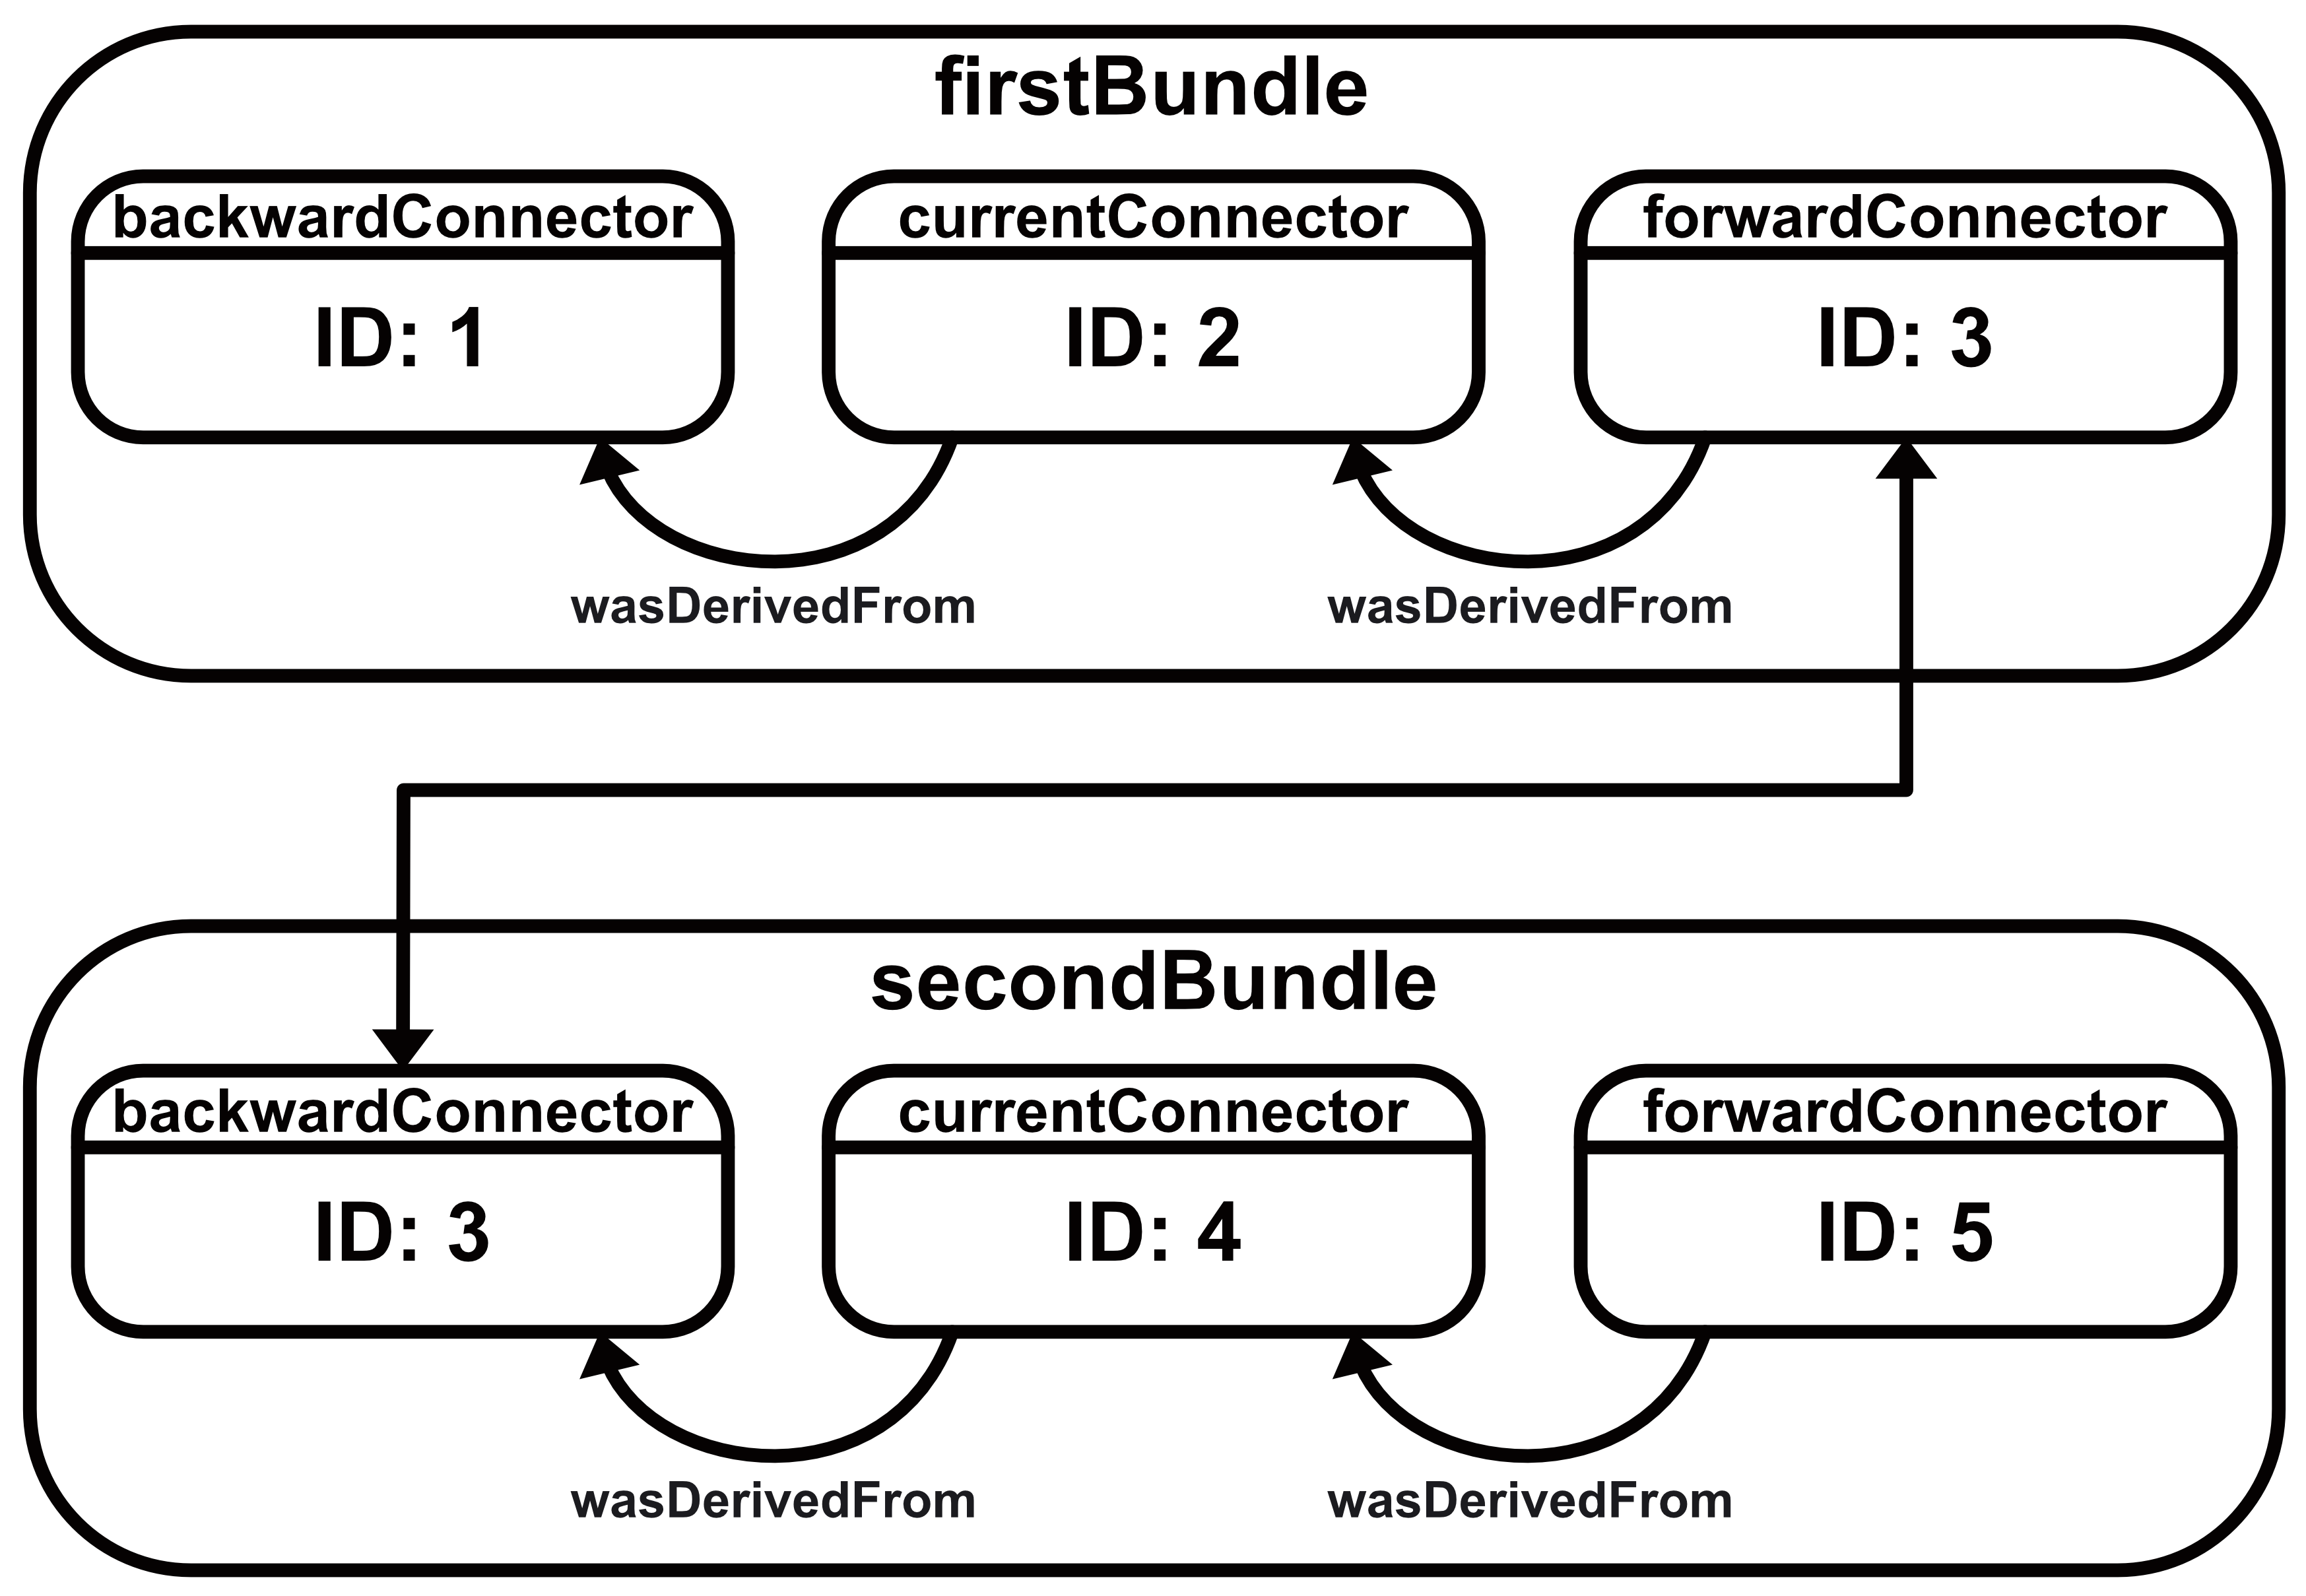
\includegraphics[width=12.5cm]{fithesis/images/bundleconnection.png}
  \end{center}
  \caption{Connection of two provenance bundles}
  \label{fig:bundleconnection}
\end{figure}

While the example simplifies the structure, it is important to note that, in practice, a single bundle can contain multiple connectors of the same type. This multiplicity allows connections to more than one Bundle on either side of the provenance backbone, thereby accommodating complex provenance scenarios.
\shorthandon{-}

\section{Real-world distribution}
The provenance chain is meant to be used in a distributed environment, meaning the whole provenance chain is distributed across multiple companies and that one or more Bundles from the chain represent a company's processing of the provenance's object, effectively documenting its complete lifecycle. An example of this would be the collection of a biological sample from a person and its subsequent processing. The first Bundle in such a chain would represent the collection center and document information such as who and how collected the sample or from whom it was collected. It would then be linked to a succeeding Bundle in the chain, representing the research center where the sample was sent. Following this formula, the whole lifecycle of the sample would be documented, making its history traceable for future verification or measurement replication.

\section{Additional concepts}
Additional concepts were developed in order to address issues that tie to the usage of the provenance chain in a distributed environment. One such issue is how to account for versioning of Bundles in the chain. To address it, the meta-provenance is used. Meta-provenance is a Bundle that keeps provenance, like the current version and its hashes, about the Bundles, ensuring that each one links to the correct version of the succeeding Bundles. 

Another issue emerged from the fact that the links pointing to Bundles in the chain can change, for example, due to changes in different versions of a Bundle. To mitigate this issue, persistent identification (PID) is used. The PID guarantees that the link to the Bundle will always be valid. This is accomplished by the PID service assigning a unique identification for the passed link and returning it to the user, who can then resolve this identification into the original link. If the original link is not valid anymore, the returned identification is assigned to the new valid link, ensuring the user always has access to the linked Bundle.

The last concept is a navigational table, which is used to store and retrieve the created PIDs. A row in this table represents a single connector Entity, and each connector Entity in each Bundle can have its own navigational table. A row in this table consists of four cells. The first cell is the identification of the Entity. The second cell is the type of connector the Entity is. The third cell identifies a Bundle to which the Entity points and the last cell identifies meta-provenance containing the pointed Bundle.

These three concepts allow the provenance chain to work in a distributed environment and are also used in the implementation.


\chapter{Design}
\shorthandoff{-}
This chapter delves into the architecture and logic of the command line tool and its underlying library, both developed as an implementation part of this thesis. The chapter has three main objectives. Firstly, it aims to provide a clear and concise overview of the implementation structure and its components, including their respective roles in its lifecycle. Secondly, it discusses the simulated environment of a real-world distribution and how it works. Finally, it describes the primary logic used to traverse a provenance chain. 
\shorthandon{-}

\section{Overview}
Thanks to its command line interface, the implementation allows users to perform different operations by entering their associated commands. The main operation is to provide the user with the ability to retrieve precursors or successors of an Entity in a provenance chain. The secondary operation is to retrieve the precursors or successors together with the main activity of their Bundles. The additional operations are to print this implementation's navigational table and to resolve data for an Entity from the mentioned table.

A bonus feature of the implemented command line interface is that it serves as a code reference for anyone who wants to use one or more library components for their project. By looking at the code of the interface, any interested party can gain insight into how and where to initialize and use the library's components for their intended results.

Furthermore, the implementation contains a secondary library used to generate meta-provenance to keep the provenance of Bundles in the chain with their hashes. This secondary library is used only for the simulation, to be described in "simulation."

\section{Structure}
\shorthandoff{-}
The implementation is designed as a modular, multi-component library. Central to this structure is a layered architecture, segregating the library operations into distinct layers - data retrieval, processing, and presentation. 

The data retrieval layer is responsible for loading and deserializing the PROV-N files, depending on the type of storage. 

The processing layer handles the traversal of the provenance chain as well as the traversal of the provenance backbone inside each PROV-N document. It is also responsible for verifying the integrity of documents and retrieving data from the navigational table and meta-provenance.

Finally, the presentation layer provides the interface for user interaction, enabling the user to enter commands and display results on the command line.
\shorthandon{-}

\subsection{Components}
\shorthandoff{-}
The library's components are separated into four main parts.
\begin{enumerate}
    \item \textbf{Main UI:}
        The Main UI component is tasked with the initialization of resources for the library and providing a user interface on the command line, where the user can input commands and view the results of the entered queries. The user interface also provides quality-of-life functions, such as command auto-completion, command history, or in-command query history.
    \item \textbf{Configuration:}
        The Configuration component retrieves data from a configuration JSON file and passes it to the library.
    \item \textbf{Tools:}
        The Tools component serves as a toolset for the library, with the first set of tools used to retrieve and deserialize PROV-N documents depending on their storage type. 
        The second set of tools is used to resolve persistent identifiers stored in the relevant navigation table.
        The third is used for retrieving hash values from the corresponding meta-provenance, and the last is used for hash creation.
    \item \textbf{Main logic:}
        The Main logic component handles the data processing. It traverses the provenance chain and retrieves the user-specified data. It also assures the correctness of the traversed chain by evaluating the integrity of the document using its hash values stored in the corresponding meta-provenance and comparing it to new hash values created using the last set of tools.
\end{enumerate}
\shorthandon{-}

\section{Simulation}
\shorthandoff{-}
For the implementation to provide a more focused simulation of a real-world environment, some limitations had to be established specifically for this thesis. The simulation of a distributed environment is performed on a set of prepared files. The thesis supervisor provided this set comprising 6 PROV-N files, each containing a single Bundle pre-filled with domain-specific data and a provenance backbone defined in "provchain" to form a provenance chain. This provenance chain represents a process from digital pathology, where a biological sample is retrieved from a patient, to be then processed for the generation of image data, which is then used as input for the training of artificial intelligence. The described process consists of 6 steps, with each step being documented in one of the Bundles from the chain. The simulation itself is achieved by a recursive call of the Main logic on this provenance chain. In contrast, in a real-world environment, this Main logic would exist, for example, in a public API of a service deployed in multiple instances. 

Because when the work on this thesis began, the concept of provenance chains was a state-of-the-art solution for the representation of distributed provenance, the way PID resolution and meta-provenance were going to work still needed to be decided. Both had to be implemented in this thesis to overcome this issue and simulate their existence in a real-world environment. For meta-provenance, a second library was implemented. This library generates a single meta-provenance containing all Bundles from the chain, along with their hashes, which it also generates using the "Tools" for hash creation. To simulate PID resolution, an in-memory implementation of a navigational table is used. This table consists of all Bundles in the chain, and access to it is implemented through the PID resolution Interface. The inclusion of this Interface allows the implemented library to be extended to other types of PID resolution and navigational tables.
\shorthandon{-}

\section{Provenance chain traversal}
\shorthandoff{-}
This section discusses the traversal of the provenance chain using the provenance backbone and retrieval of precursors or successors of an Entity. The inputs for this traversal are a QualifiedName identifier of an Entity and a QualifiedName identifier of a Bundle containing the Entity. In this example, the traversal moves in a forward direction, retrieving the successors of the Entity. The successors are represented by backwardConnectors. The inputs are prefix1:entity1, which is a forwardConnector from prefix1:bundle1, and the provenance chain has a structure, as shown in "Figure."

\begin{figure}[htbp]
  \begin{center}
    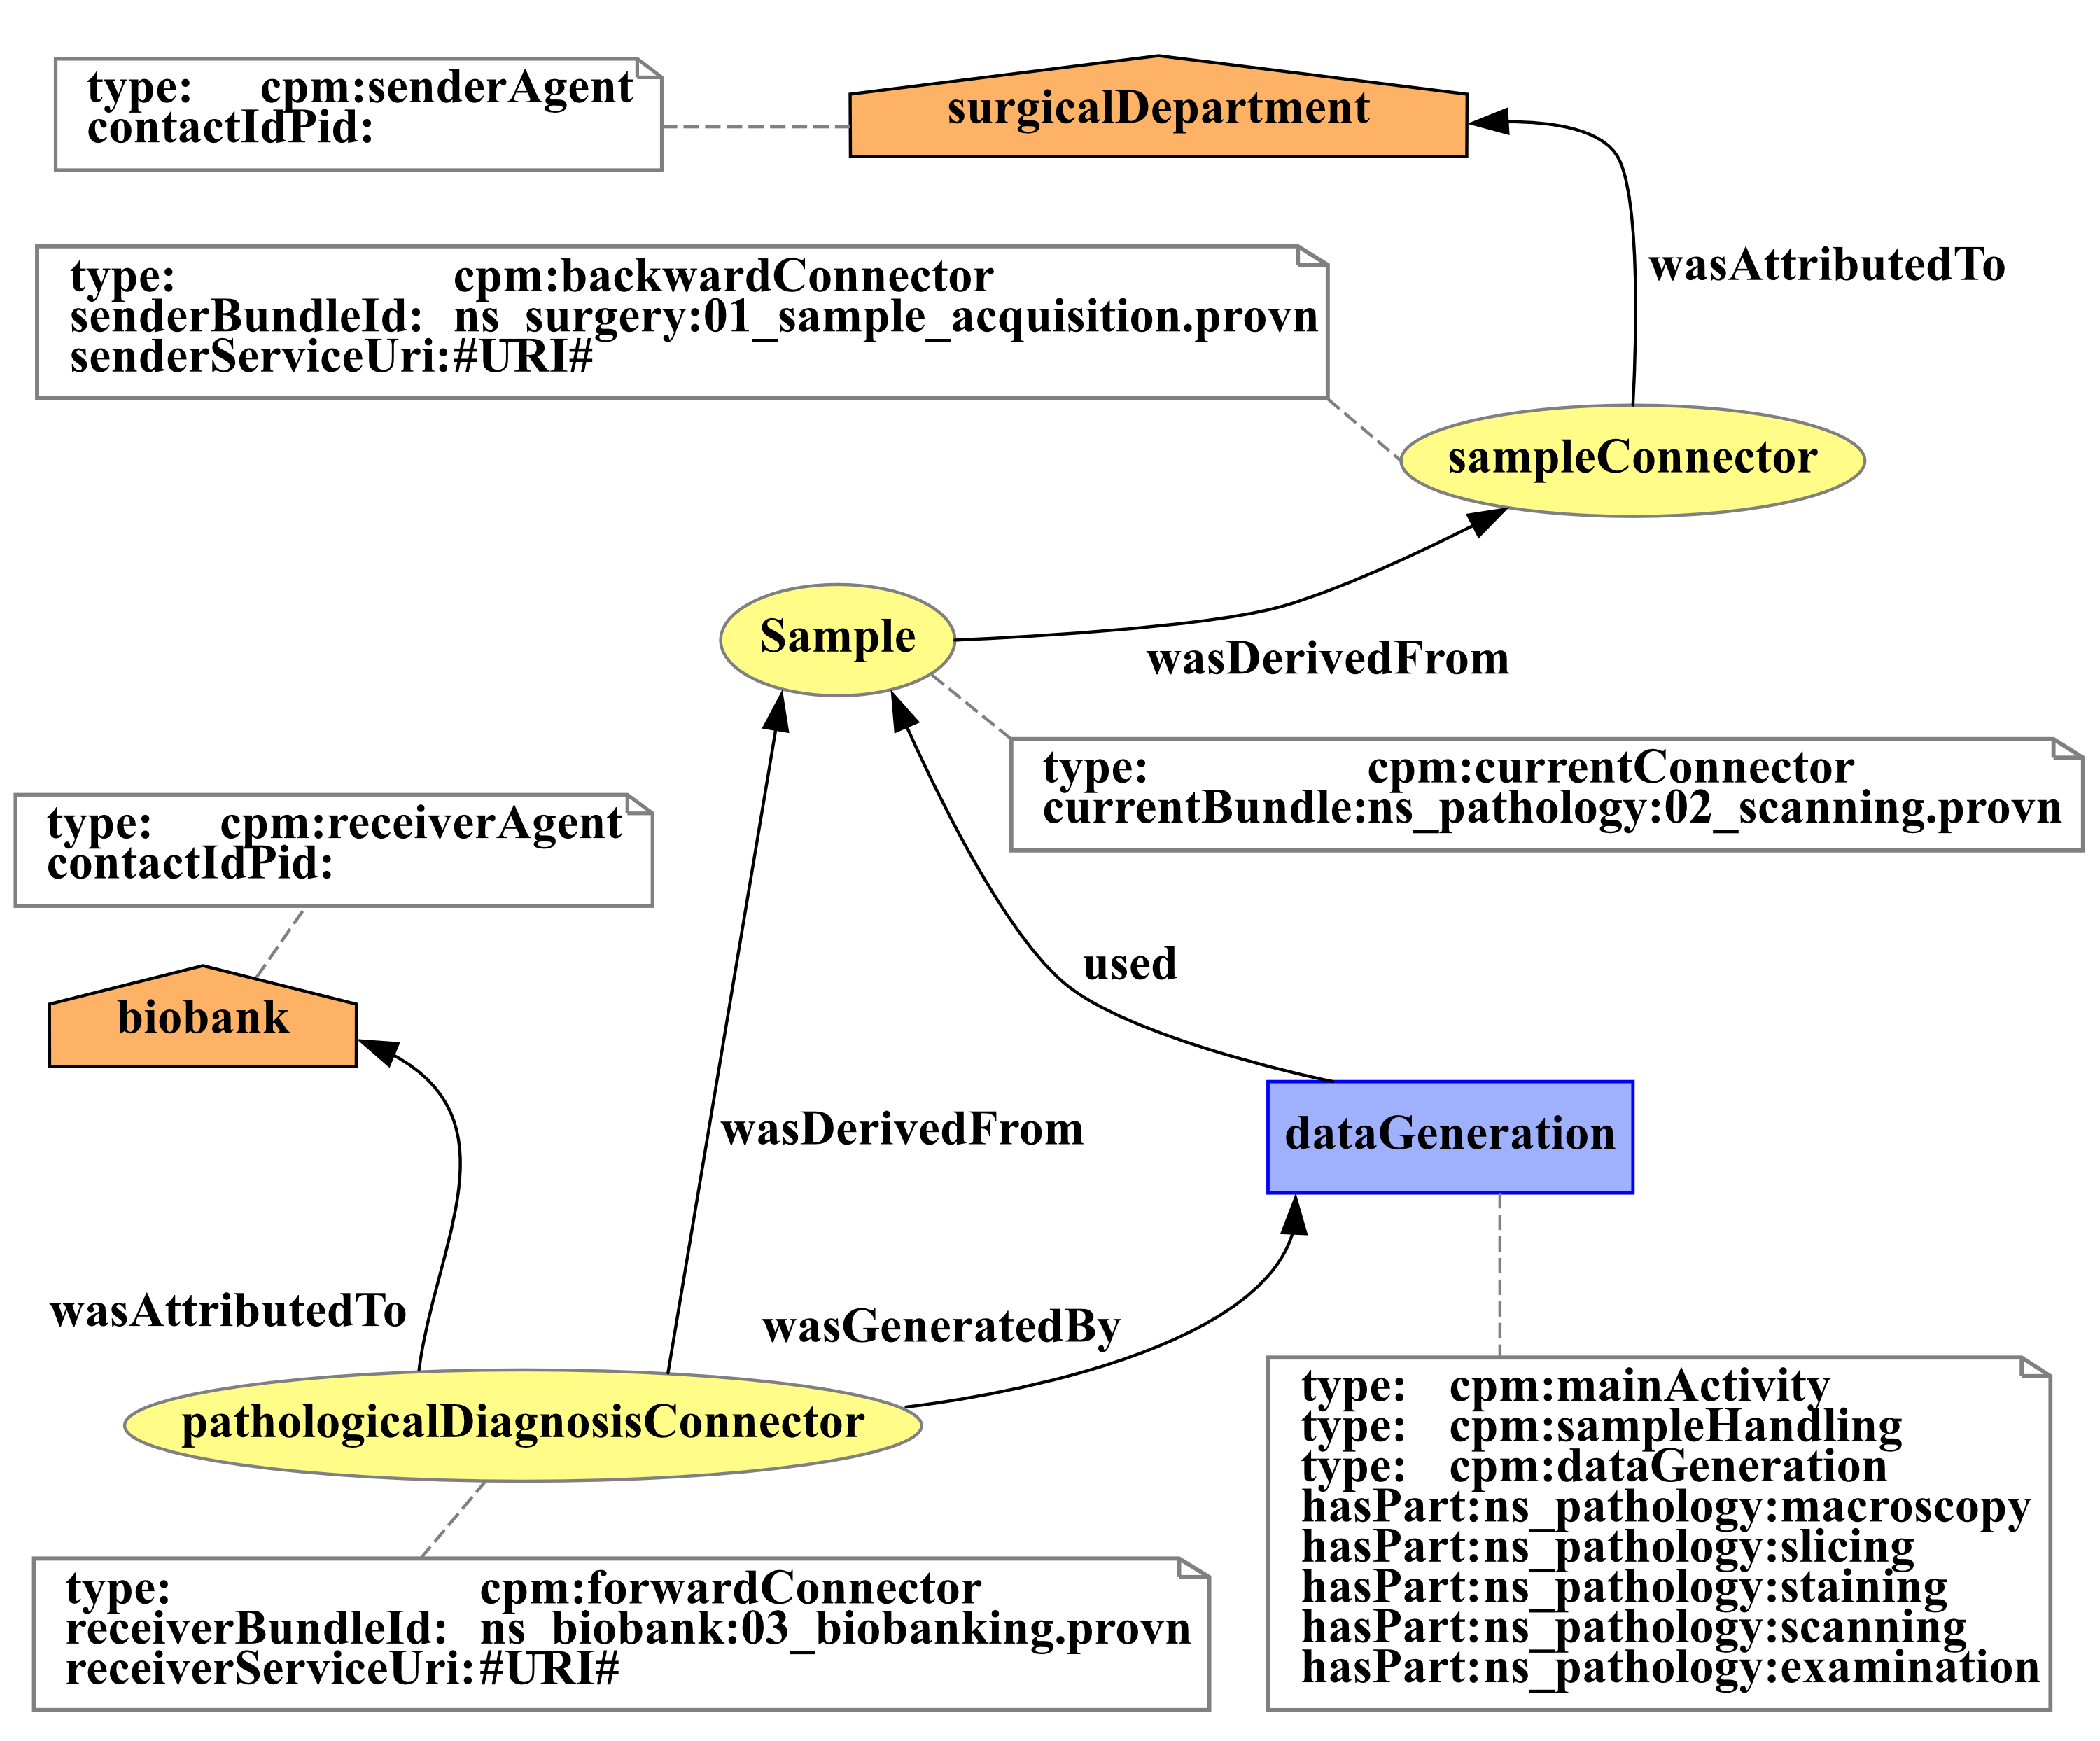
\includegraphics[width=9cm]{fithesis/images/examplebigger.png}
  \end{center}
  \caption{Example provenance chain structure}
  \label{fig:bundleexample}
\end{figure}
\shorthandon{-}

Considering the traversal is already at the end of the bundle1's backbone, the next step is to move to the Entity linked to the entity1, which is an Entity with the same identifier in the bundle2.

\begin{figure}[htbp]
  \begin{center}
    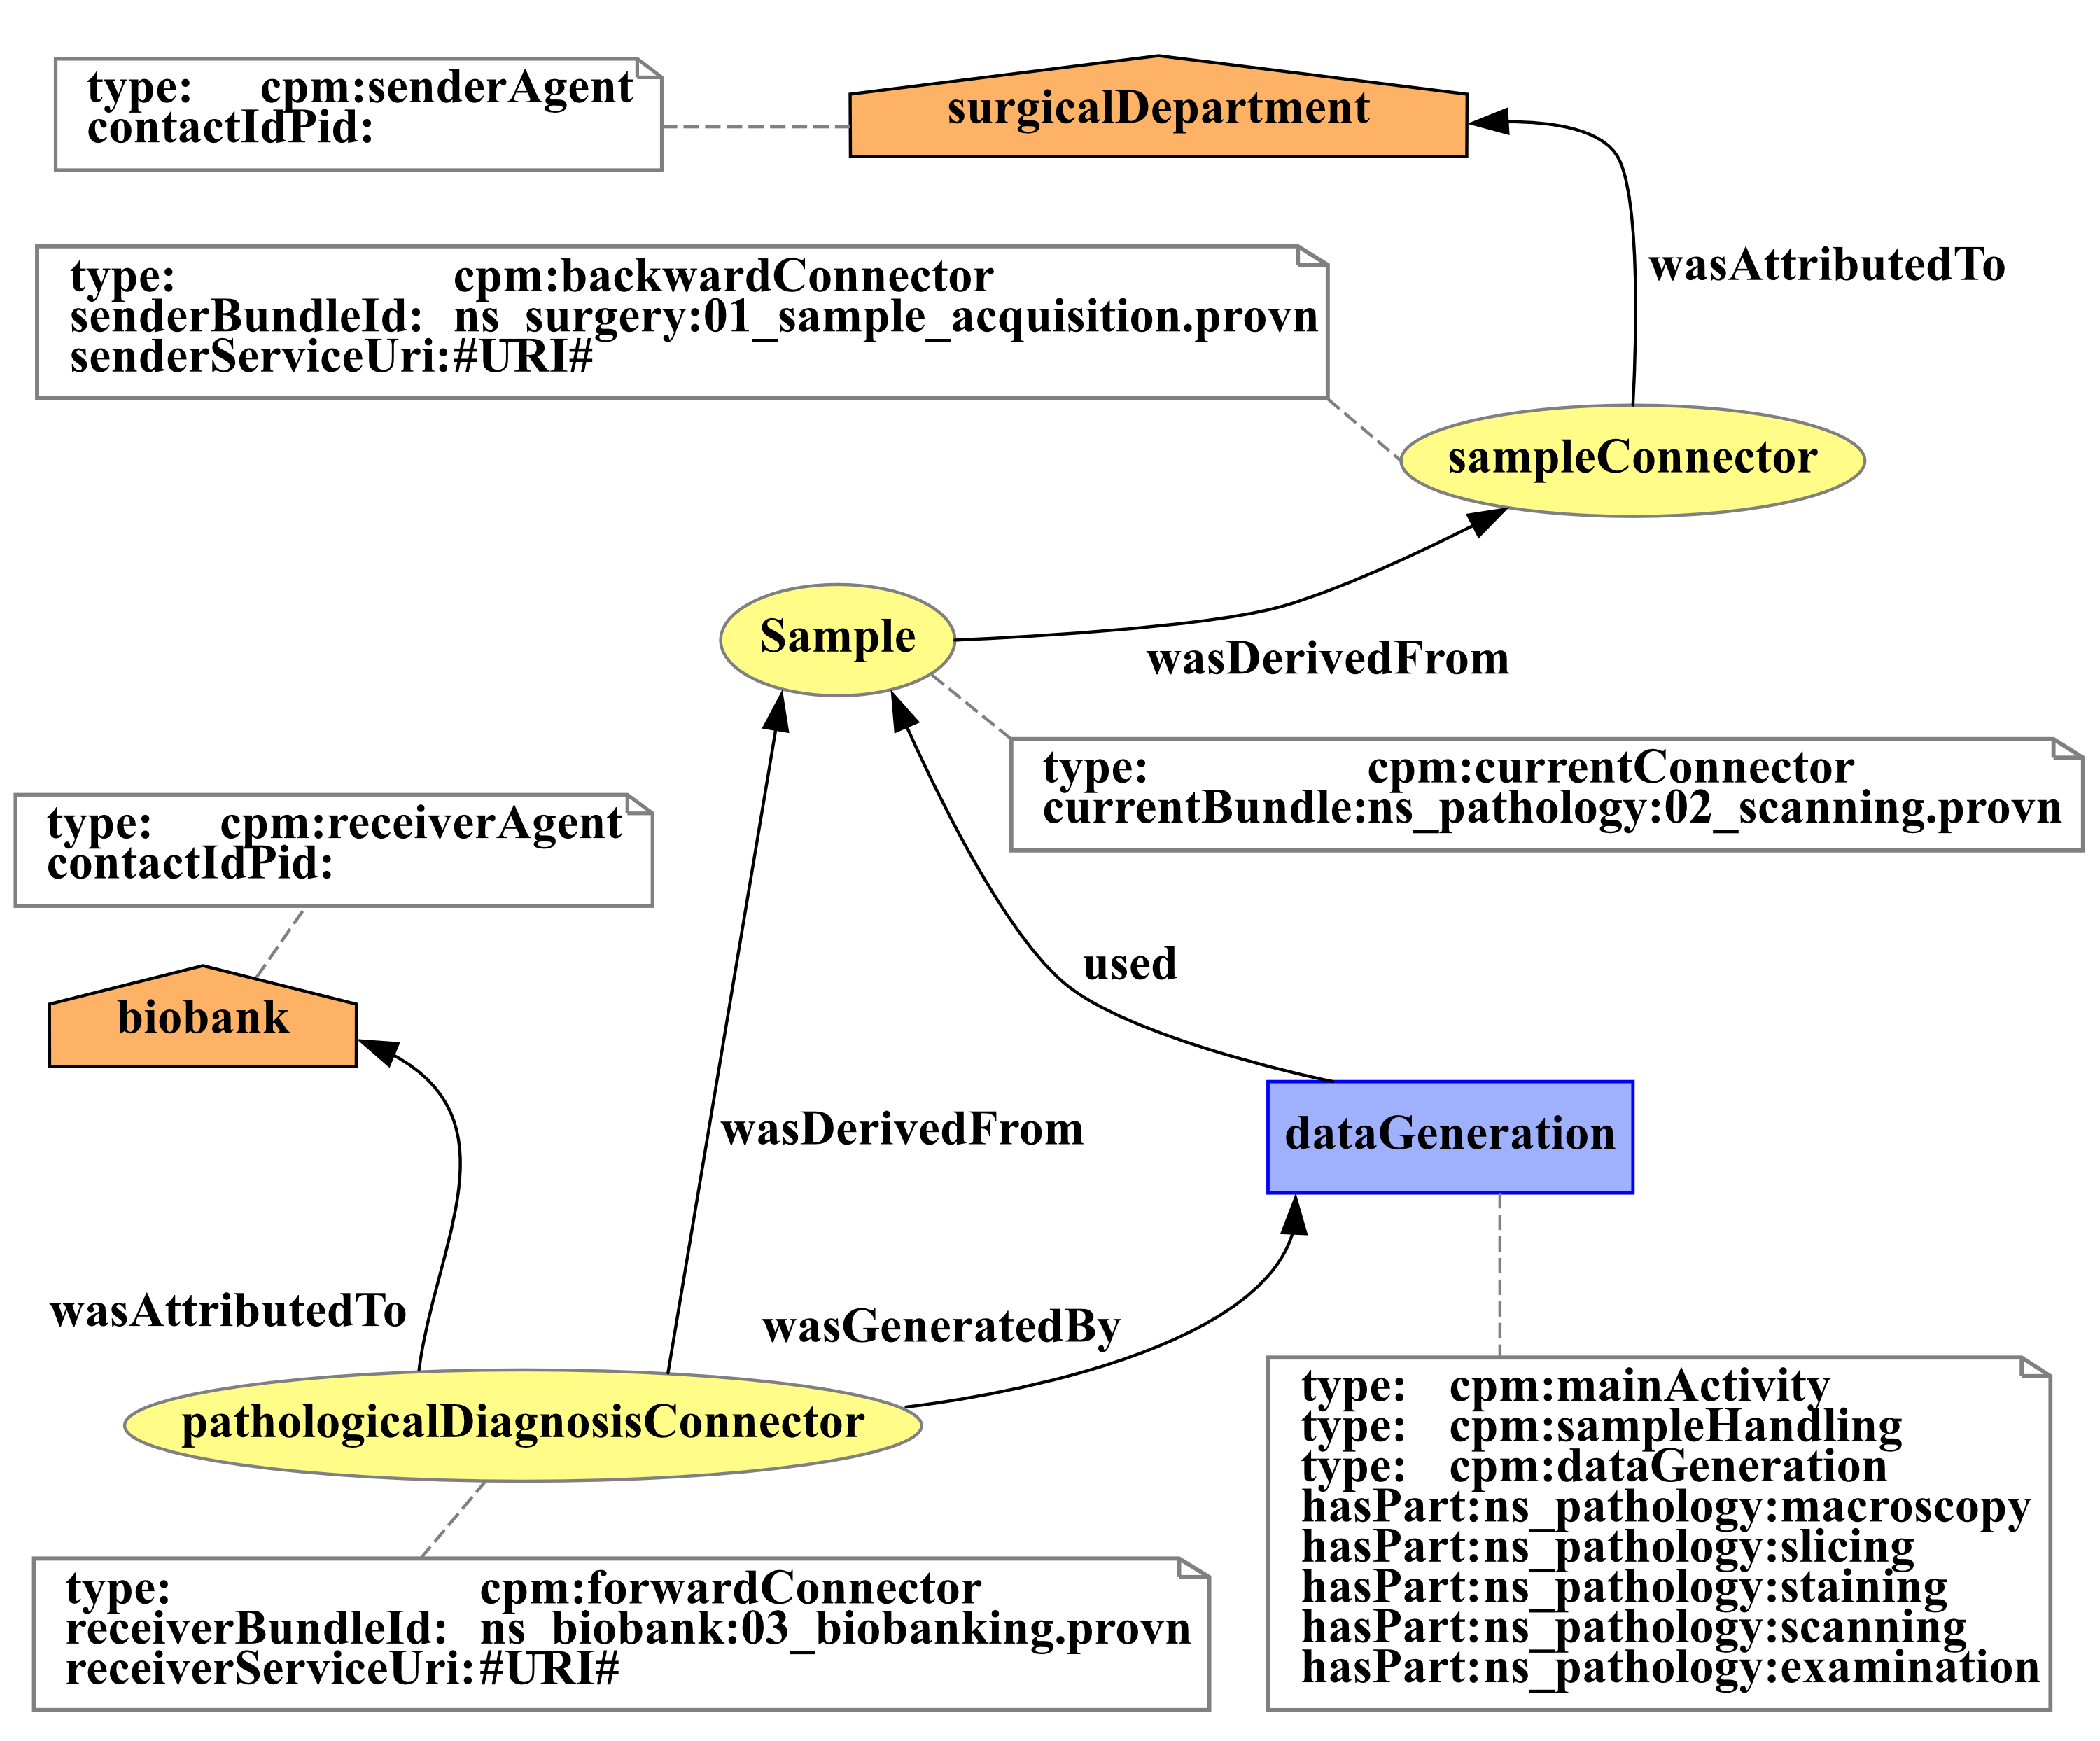
\includegraphics[width=9cm]{fithesis/images/examplebigger.png}
  \end{center}
  \caption{Moving between Bundles}
  \label{fig:bundleexample2}
\end{figure}

Because the traversal is currently on a backwardConnector, the current Entity and Bundle identifiers are returned, and the traversal continues.

\begin{figure}[htbp]
  \begin{center}
    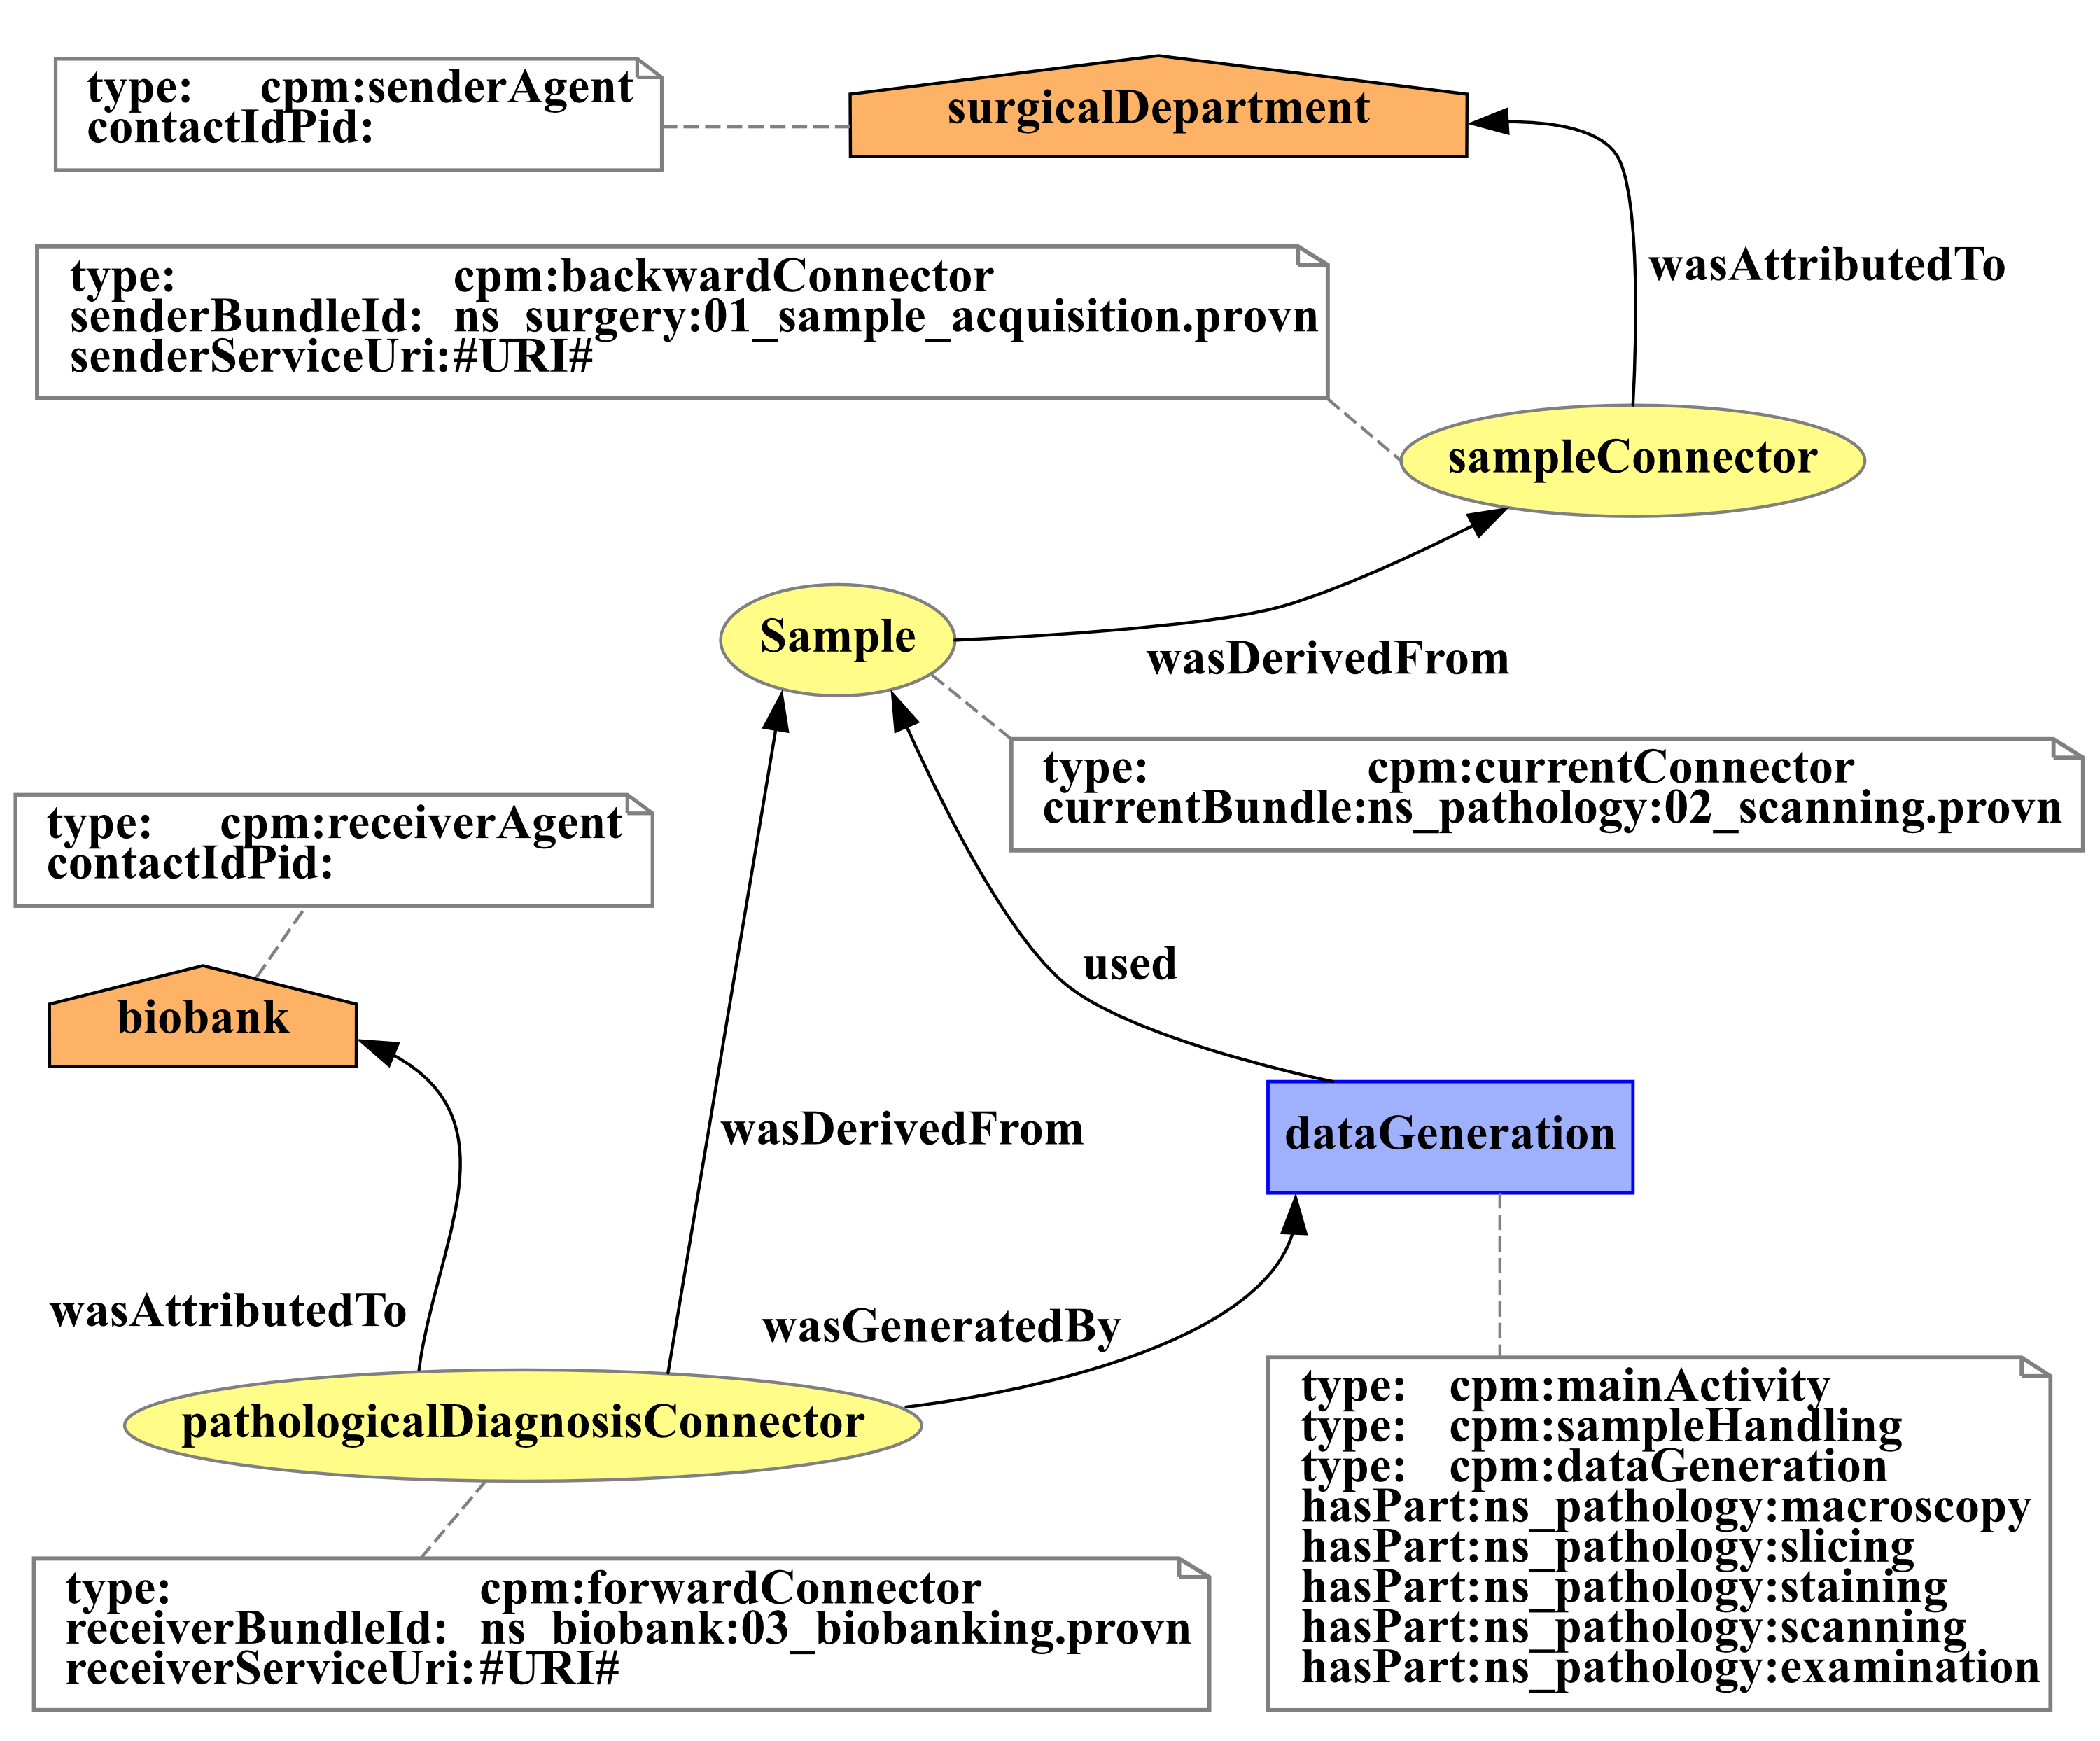
\includegraphics[width=9cm]{fithesis/images/examplebigger.png}
  \end{center}
  \caption{QualifiedNames of the current Entity and Bundle}
  \label{fig:bundleexample3}
\end{figure}

The next step is for the traversal to move using the wasDerivedFrom edge onto the following Entity, which is a currentConnector, and then move again using the wasDerivedFrom edge to arrive on a forwardConnector. The traversal moves into the next Bundle, and the whole process repeats, retrieving the next successor.

\begin{figure}[htbp]
  \begin{center}
    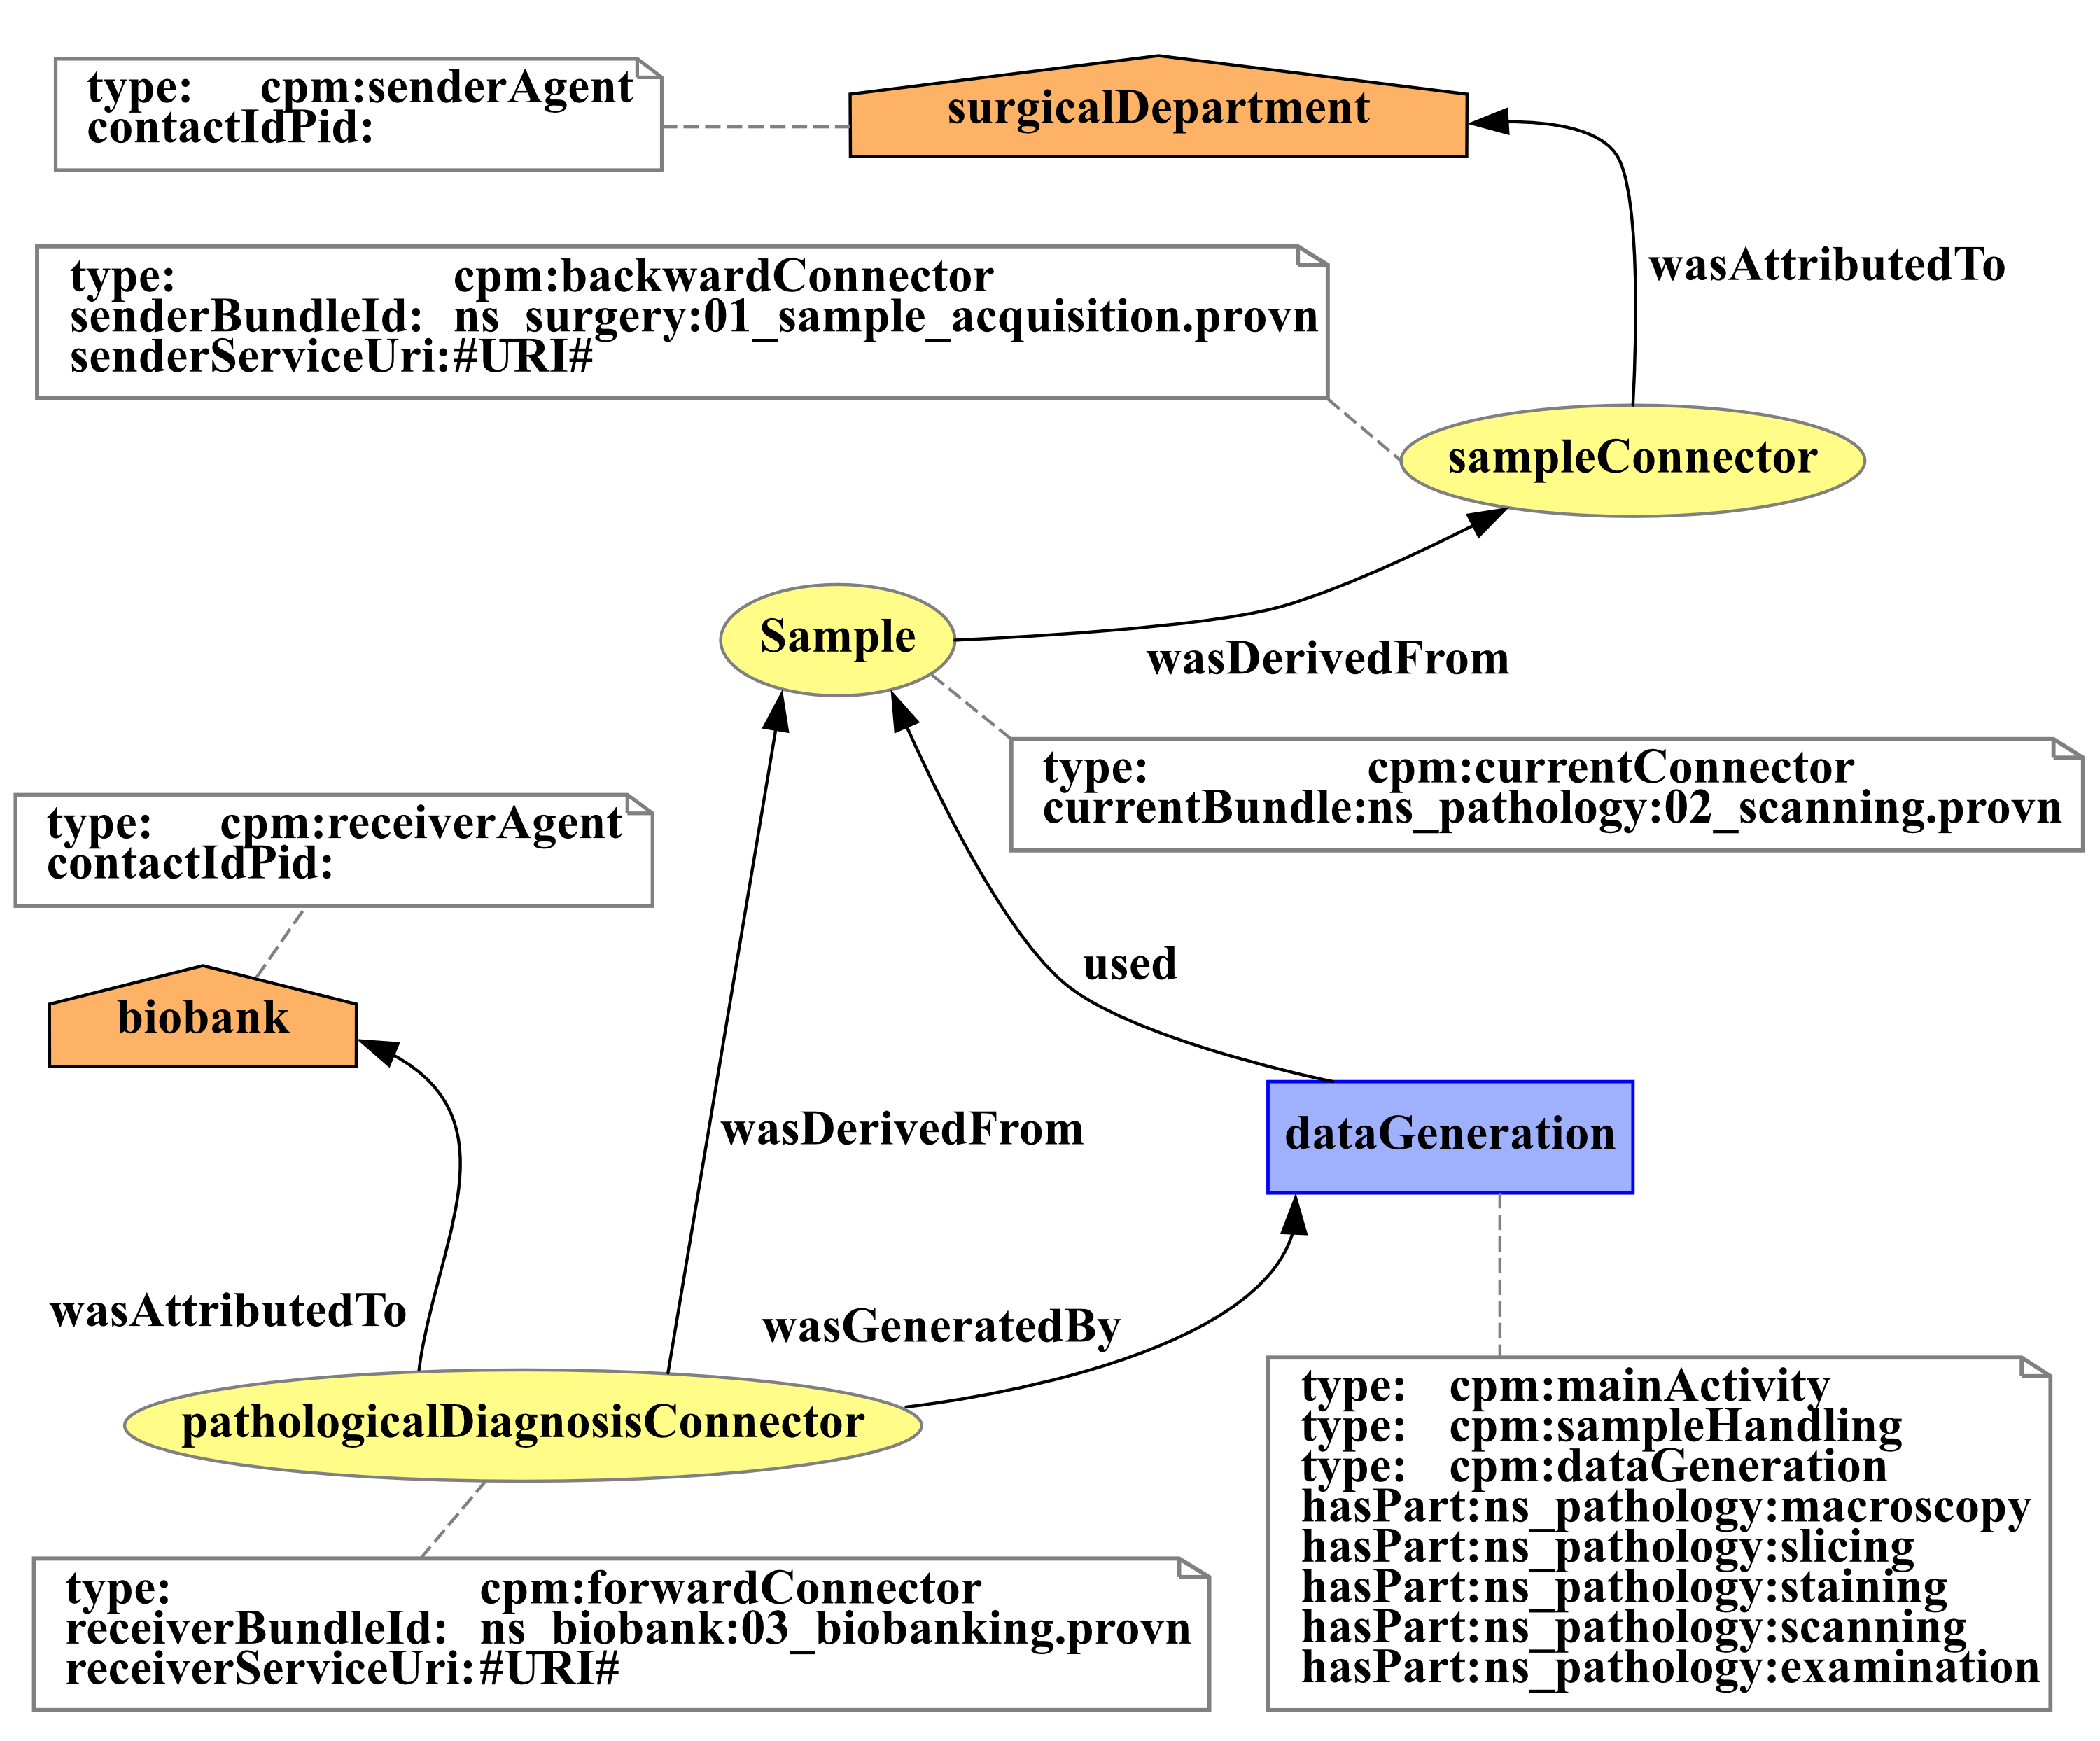
\includegraphics[width=9cm]{fithesis/images/examplebigger.png}
  \end{center}
  \caption{Traversal of the Bundles backbone}
  \label{fig:bundleexample4}
\end{figure}

The traversal ends when no more Entities are derived using the wasDerivedFrom edge, or there are no succeeding bundles.


\chapter{Implementation}
\shorthandoff{-}
This chapter aims to bridge the gap between the theoretical framework outlined in the Design chapter and the actual realization of the project. It offers an in-depth look at the code structure, libraries used, and the problems that arose during the implementation. Through a clear and systematic presentation, this chapter showcases the application's development process and serves as a valuable resource for understanding the practical challenges and solutions encountered. Reading this chapter will offer insights into the application's architecture and operational mechanics, providing a deeper appreciation of the project's technical complexity.

\section{Project structure}
TODO

\section{Used technologies}
The following part delves into the libraries and tools used in the implementation and the reasoning behind each.
\subsection{ProvToolBox}
ProvToolBox is a library for managing provenance data. This implementation uses it's two sub-libraries prov-model and prov-interop-light.  
The prov-model is used across the whole library to create and manipulate provenance documents.
Complementary to the prov-model, the prov-interop-light enhances the system's interoperability. This library facilitates the conversion of provenance data into various formats, ensuring that the application can communicate effectively with other provenance-aware systems and tools.
\subsection{Jackson Databind}
Jackson Databind is a library for handling JSON data formats. In ConfigLoader.java and Configuartion.java, 'jackson-databind' parses the configuration file and creates Java objects from JSON. This functionality is crucial in managing configurations within the library.
\subsection{GitLab4J API}
Integrated primarily in GitLabFileLoader.java, the GitLab4J API is a library to facilitate interaction with GitLab's APIs. It automates file retrieval, allowing the library to support git-based provenance storage.
\subsection{JLine Bundle}
JLine Bundle is a library used to enhance the user interface of the implementation, as seen in MainRuntime.java. It provides capabilities such as command-line completion and history, significantly improving the user experience by making the interface more intuitive and responsive.
\subsection{Jansi}
Utilized in MainRuntime.java, Jansi is a library used to add stylistic improvements to the console output. It renders text in different colors and styles, making the console output about the integrity of Bundles more readable and user-friendly.
\subsection{Apache Maven Shade Plugin}
Including the Maven Shade Plugin plays a significant role in the library's build process. This plugin creates an uber-jar, a standalone executable jar file containing all the necessary dependencies. This approach simplifies deployment and distribution, ensuring the library is self-contained and can be run in diverse environments without additional dependency management.


\section*{}
Each library has been chosen and integrated into the implementation to address specific functional requirements and enhance the application's usability, efficiency, and interoperability. The strategic use of these libraries aligns with the broader goal of creating a user-focused, adaptable, and future-proof application.

\section{Runtime}
This section is intended to provide a concise runtime walkthrough of the library. The purpose is to offer insight into how different classes and components interact to produce the desired query results for the user. By following this walkthrough, readers will understand the underlying mechanisms of the library's runtime operation. Starting with the class Main, which serves as a single entry point, calling the static MainRuntime class. MainRuntime serves as the top-level part of the library, statically initializing all resources and simultaneously providing a user interface for command inputs.

For this walkthrough, the queried request is to retrieve the precursors of an Entity by using the 'precursors' command. In the context of the 'precursors' command, i.e., when traversing the provenance chain backward, the mentioned precursors are represented as forwardConnector Entities of the preceding bundles.

After the command is identified, the findPrecursors method is entered with a false argument, as the user does not wish to retrieve the main Activity alongside the precursors. Upon entering the method, the user is prompted to enter the Entity's ID and URI and the ID and URI of the Bundle in which the Entity resides. Next, the correct implementation of the IFileLoader interface is chosen to retrieve the PROV-N file and return it deserialized into a Document object. After that, the integrity of the Document is verified by calling the checkSum method of the Crawler class. With this, the preparation phase ends, and the runtime enters the Crawler's method getPrecursors.

Upon entering, the proper navigational table resolver is chosen, and the connector type of the Entity is retrieved. Next comes the first if branch, checking whether the connector type is a forwardConnector. If not, the method continues; if it is, the current Entity with its Bundle is retrieved as a precursor, and the method continues. Right after the first if branch comes a second one checking whether the connector type is a backwardConnector; if it is, it means the method reached the end of the current Bundle's graph, and it will repeat the same process as in the MainRuntime section, retrieving the following Document and verifying its integrity after which, it calls the getPrecursors method recursively. If not, it will search through the WasDerivedFrom statements in the Document to find which Entity is following in the traversal and call the getPrecursors method recursively with the same Document and the newly found Entity. 

After the runtime is done traversing every Bundle in the chain, it prints those results on the command line, along with confirmation of the verified integrity of each Bundle.

\section{Problems during implementation}
Four main problems were encountered during the implementation due to using the ProvToolBox Java library. The simulation files provided by the supervisor were generated using a Python library, which produced files with some notation differences. The first is that the Python library supports attributes with multiple values using parentheses, while the Java library needs each attribute to have only one value.

\begin{verbatim}

    Python: 
        dct:hasPart=('prefix:local','prefix:local')
    Java:
        dct:hasPart='prefix:local', 
        dct:hasPart='prefix:local' 
        
\end{verbatim}

The second problem came from the Python library supporting the creation of Entities with space in names, which is seen as a syntax error by the Java library.

\begin{verbatim}

    Python:
        entity(prefix:local 1, [prov:type=...
    Java:
        entity(prefix:local_1, [prov:type=... 
        
\end{verbatim}

The third problem was caused because the Python library generates attributes with values encompassed by double quotes. The Java library differentiates between single and double quotes. The single quotes are resolved as the QualifiedName specified inside of them.

\begin{verbatim}

    cpm:receiverBundleId='prefix:local.provn'
    
    Resolved:
        'prefix:{{uri}}local.provn'
        
\end{verbatim}

While the double quotes are regarded as a LangString

\begin{verbatim}

    cpm:receiverServiceUri="#URI#"
    
    Resolved:
        LangString@xxx[value=#URI#,lang=<null>]
        
\end{verbatim}

The last problem came from the fact that the ProvToolBox library, at the time of thesis implementation, was left on version 0.9.3, with the last update being over a year ago, which caused some of the library's features not to work correctly or at all. As of the late summer of 2023, the development seems to have returned, and new updates are being released.
\shorthandon{-}


\chapter{Manual}
\shorthandoff{-}
\section{Set-up}
To utilize the library, it is necessary to have Maven and Java properly configured. To simplify the process for users, the implementation is currently spread across multiple Git repositories, including two on FI and ICS GitLab sites and one on the author's personal GitHub page. To obtain the library, clone the repository or use the download button to retrieve the entire repository bundled in a zip or another archive file.

\subsection{Retrieving the repository}
In order to clone a repository, it is important to confirm that Git is installed on the device. Following this, proceed to the repository's page on GitLab or GitHub and locate the "Clone" button. A URL to copy will be generated by clicking on this button. Next, launch the terminal or command prompt, navigate to the directory where the repository should be stored, and execute the command 'git clone [URL]', replacing [URL] with the URL you copied earlier. Doing this will generate a local copy of the repository on the device. If cloning is not possible, an alternative is to download the repository as a ZIP file. On the repository's page, look for the "Download ZIP" option, typically found in the same section as the clone option. Clicking on this will download the repository's contents in a compressed file, which can then be extracted to the preferred location.

\subsection{Simulating the environment}
The initiation of simulation files is the first step in simulating an environment, which requires the retrieval of specific files necessary for the simulated environment to function effectively. To achieve this, the cloned repository should be opened in the console. The submodule can be navigated by using the command.

\begin{verbatim}
$ cd. \src\main\resources\bthesis-provenancechain-digpat  
\end{verbatim}

Once the submodule is reached, the command 

\begin{verbatim}
$ git submodule foreach git fetch –tags
\end{verbatim}

should be executed. After it finishes, there should be no output. Finally, the command

\begin{verbatim}
$ git submodule update --init --recursive  
\end{verbatim}

should be run to conclude the process. This will ensure that the bthesis-provenancechain-digpat submodule contains the required .provn files.

\section{Building}
The jar file is packaged using the Maven Shade plugin, which is the preferred method. To create the jar file, navigate to the cloned repository using the console and run the \textbf{\texttt{'mvn clean package'}} command. After creating the jar file, it can be launched by executing the command \textbf{\texttt{'java -jar }\path{.\target\BThesis-ProvenanceChain-VERSION-shaded.jar'}}. In the event that the intended environment does not have a JRE, the \textbf{\texttt{'jpackage'}} command line tool provided by Java can be used to create a platform-specific installer.

\section{Omitting the simulated environment}
To facilitate traversal simulation, the implementation employs several classes and files that provide the necessary objects for the algorithm to function. These classes have been transferred to packages labeled 'bthesis.provenancechain.simulation' and 'bthesis.metageneration' to enhance clarity. At the same time, the required files reside in the previously mentioned submodule 'src.main.resources.bthesis-provenancechain-digpat'. However, these components can be omitted if the required classes are adequately substituted.
\shorthandon{-}


\chapter*{Conclusion}
\markright{\textsc{Conclusion}}
\addcontentsline{toc}{chapter}{Conclusion}
\shorthandoff{-}
Lorem ipsum dolor sit amet, consectetur adipiscing elit. Integer finibus commodo leo. Nullam blandit imperdiet magna, sit amet tempor tortor sagittis vitae. Lorem ipsum dolor sit amet, consectetur adipiscing elit. Cras elementum diam vel eros tristique, at maximus tortor ultricies. Curabitur urna magna, dictum at porta rutrum, congue nec justo. Nam ac rhoncus lectus. Ut feugiat volutpat ornare. Mauris quis neque nec lorem vestibulum iaculis. Proin posuere nisi eget nisi tristique, eu tempus nibh ultricies.
\shorthandon{-}

After linking a bibliography data\-base files to the document using
the \verb"\"\texttt{thesis\discretionary{-}{}{}setup\{bib\discretionary{=}{=}{=}%
\{\textit{file1},\textit{file2},\,\ldots\,\}\}} command, you can
start citing the entries. This is just dummy text
\parencite{borgman03} lightly sprinkled with citations
\parencite[p.~123]{greenberg98}. Several sources can be cited at
once: \cite{borgman03,greenberg98,thanh01}.
\citetitle{greenberg98} was written by \citeauthor{greenberg98} in
\citeyear{greenberg98}. We can also produce \textcite{greenberg98}%
\ or %% Let us define a compound command:
\def\citeauthoryear#1{(\textcite{#1},~\citeyear{#1})}%
\citeauthoryear{greenberg98}%
. The full bibliographic citation is:
\emph{\fullcite{greenberg98}}. We can easily insert a bibliographic
citation into the footnote\footfullcite{greenberg98}.

\printbibliography[heading=bibintoc]

\end{document}
